\section{Circuit design}
\label{sec:circuits}

All cells were designed at transistor level in the \texttt{vernier2d} library
using the \SI{2}{\volt} devices of the \texttt{tsmc18} library
(\texttt{nmos2v}/\texttt{pmos2v}, Spectre models \texttt{nch}/\texttt{pch}) at
the minimum channel length $L=\SI{180}{\nano\meter}$.
The unit inverter used throughout is $W_p/W_n = \SI{440}{\nano\meter}/\SI{220}{\nano\meter}$;
larger drivers are built as parallel fingers (multiples) of this unit.
Table~\ref{tab:cells} summarizes the cell inventory; the per-cell width budget
is given in Appendix~\ref{app:sigmaw}.

\begin{table}[H]
\centering
\small
\caption{Cell inventory of the TDC core with device sizing. All lengths
\SI{180}{\nano\meter} except the MOSCAPs (\SI{250}{\nano\meter}).}
\label{tab:cells}
\begin{tabularx}{\textwidth}{l c X}
\toprule
\textbf{Cell} & \textbf{Count} & \textbf{Contents and sizing} \\
\midrule
\texttt{delay\_tau1} & 11 &
FO=1 inverter pair ($10\times$ input, $10\times$ driver, unit
$440/\SI{220}{\nano\meter}$); MOSCAP's for trimming: three TG-switched trim banks of
$2/20/21$ fingers and one fixed TG-MOSCAP ($7/18$ fingers) connection to ensure $\tau_1=\tau_2+15\mathrm{ps}$. \\
\texttt{delay\_tau2} & 7 &
identical active devices as \texttt{delay\_tau1}; lighter trim banks of
$2/14/18$ fingers. \\
\texttt{srlatch} & 60 &
13 transistors: two 2-input NANDs (all devices
$440/\SI{180}{\nano\meter}$), asynchronous-reset NMOS
($2.0/\SI{0.18}{\micro\meter}$), two unit-inverter output buffers. \\
\texttt{nand} & (in latch) &
two series NMOS, two parallel PMOS, all $440/\SI{180}{\nano\meter}$. \\
\texttt{Inv\_10x/20x/40x/80x} & trees &
input and reset distribution buffers, parallel-finger multiples of the unit
inverter. \\
\bottomrule
\end{tabularx}
\end{table}

\subsection{Delay stage}
\label{sec:delaycell}

\begin{figure}[H]
\centering
\begin{subfigure}[t]{0.58\textwidth}
  \centering
  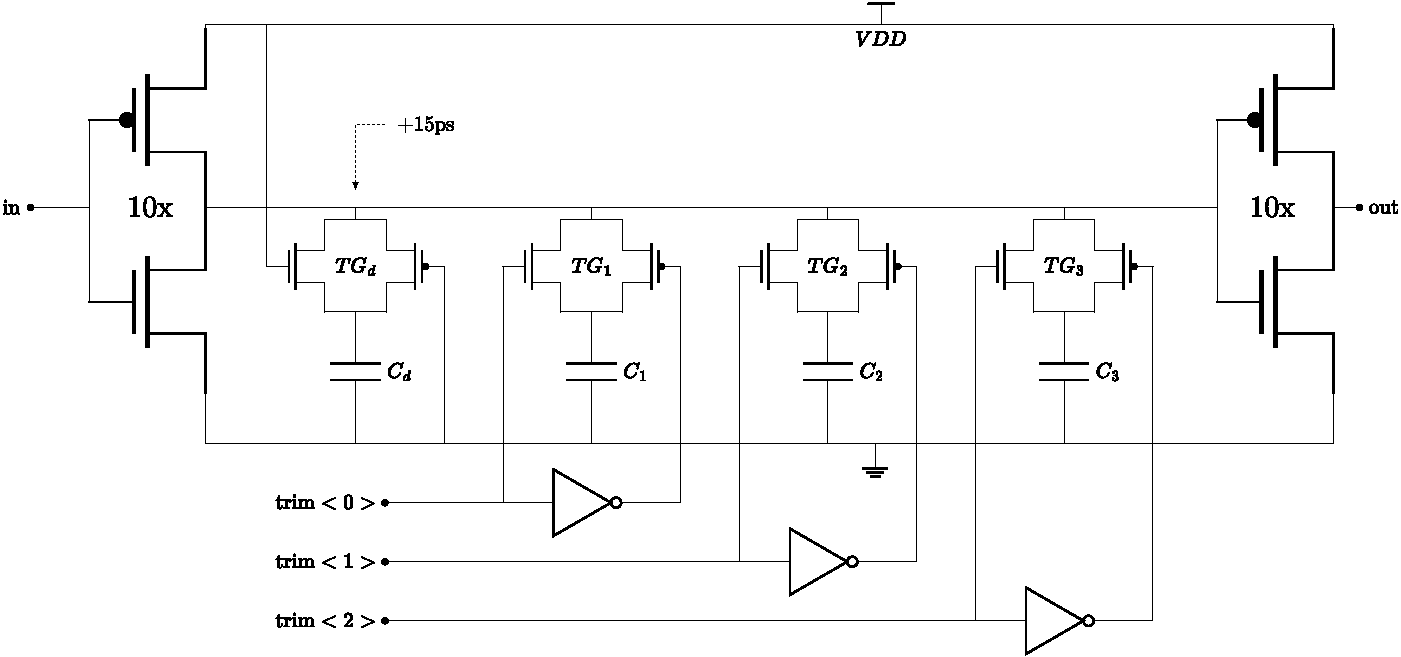
\includegraphics[width=\textwidth]{figures/delay_tau1.pdf}
  \caption{\texttt{delay\_tau1} (START line, \SI{90}{\pico\second}).}
  \label{fig:tau1}
\end{subfigure}\hfill
\begin{subfigure}[t]{0.40\textwidth}
  \centering
  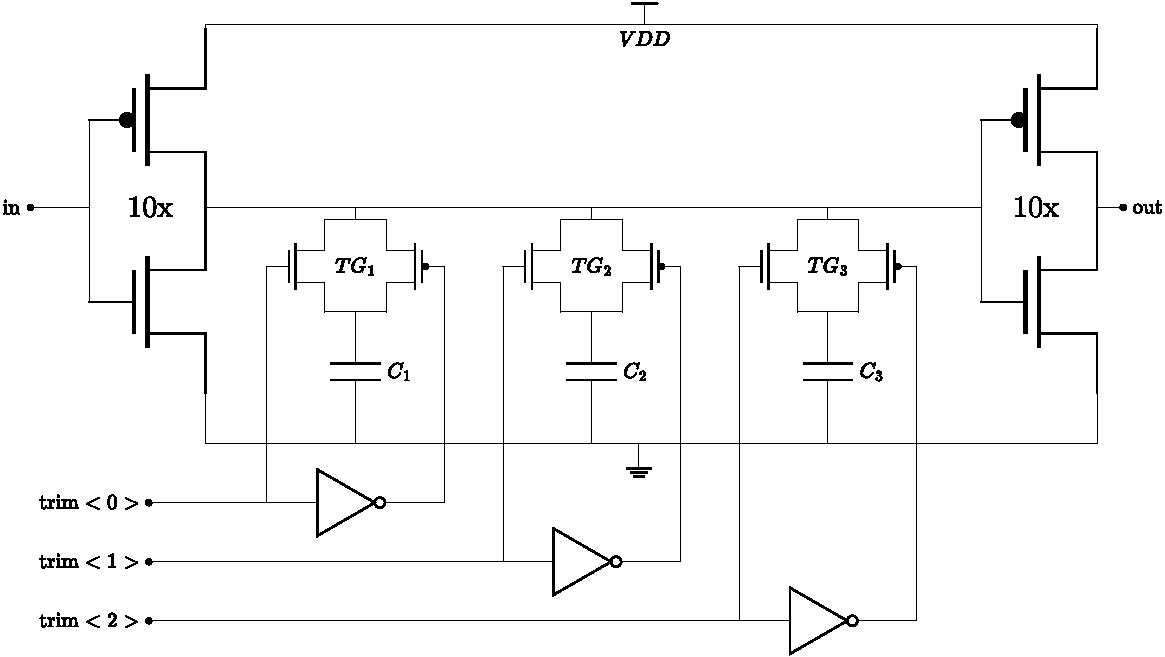
\includegraphics[width=\textwidth]{figures/delay_tau2.pdf}
  \caption{\texttt{delay\_tau2} (STOP line, \SI{75}{\pico\second}).}
  \label{fig:tau2}
\end{subfigure}
\caption{Delay stages. An FO=1 inverter pair drives the next stage; the
internal node carries one fixed MOSCAP behind an always-on access transistor
plus three transmission-gate-switched MOSCAP banks controlled by
\texttt{trim<0:2>}. The two cells differ only in bank sizes.}
\label{fig:delaycells}
\end{figure}

The delay stage is a two-inverter buffer whose internal node is loaded
capacitively (Fig.~\ref{fig:delaycells}). Two choices define it.

\textbf{Fan-out of one.} Conventional FO=4 sizing minimizes the delay of a
logic path, but here delay is the product, not the cost. With FO=4 the
intrinsic delay of the internal node pins the minimum achievable stage delay at
\SI{97}{\pico\second} in this technology, which already exceeds the required
$\ttau{2}$. Equal input and driver sizing ($10\times$ and $10\times$ unit
fingers) reduces the internal-node capacitance and opens a usable window of
\SIrange{74}{147}{\pico\second} under the true grid load.

\textbf{Capacitive tuning, identical actives.} Both lines use the same active
devices; only the capacitance on the internal node differs. The fixed MOSCAP
($18\times$ fingers, $L=\SI{250}{\nano\meter}$) sets the nominal delay, and
three banks ($2/20/21$ fingers on the $\ttau{1}$ cell,
$2/14/18$ on the $\ttau{2}$ cell) are switched in or out through transmission
gates by the static \texttt{trim<0:2>} inputs. Because both delays have the same $10\times, FO=1$ sizing, $\ttau{1}$ and $\ttau{2}$ track
each other over process and temperature, which is what keeps their difference,
the LSB, stable. At the tuned typical-corner point the lines measure
$\ttau{1}=\SI{90.5}{\pico\second}$ and $\ttau{2}=\SI{75.4}{\pico\second}$.

\subsection{Arbiter}
\label{sec:arbiter}

\begin{figure}[H]
\centering
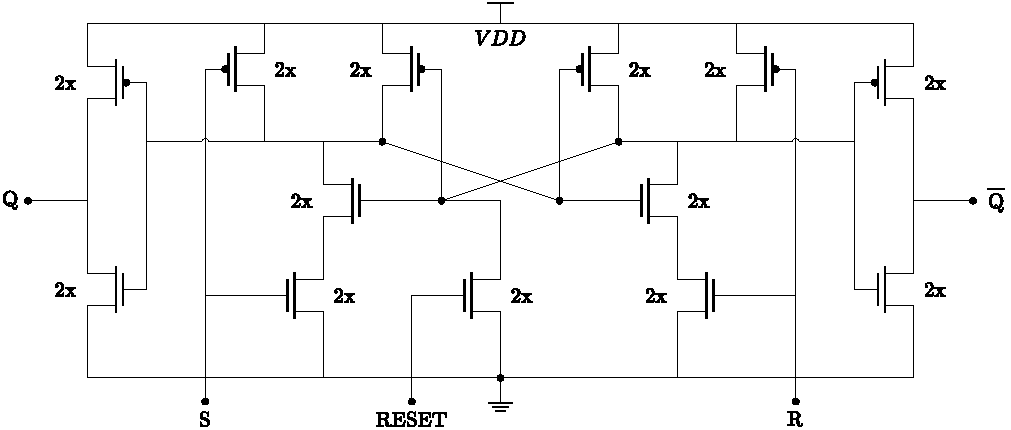
\includegraphics[width=0.8\textwidth]{figures/srlatch.pdf}
\caption{SR-latch arbiter (\texttt{vernier2d/srlatch}). Two cross-coupled
NANDs ($440/\SI{180}{\nano\meter}$ throughout), an asynchronous-reset NMOS on
the internal node, and two unit-inverter output buffers. S and R are active
high; the first rising edge wins.}
\label{fig:srlatch}
\end{figure}

The arbiter decides, at each grid node, which edge arrived first. We use a
cross-coupled NAND SR latch with buffered outputs (Fig.~\ref{fig:srlatch}),
13 transistors in total. Both NAND outputs idle high; the first rising input
flips the latch and positive feedback locks the decision. Three properties
motivated the choice over a D flip-flop. The cell is small, which matters at
60 instances. The S and R paths are electrically symmetric with equal NMOS and
PMOS widths, which is what keeps the arbitration offset at the femtosecond
level measured in Section~\ref{sec:meta}. And reset costs a single NMOS
($2.0/\SI{0.18}{\micro\meter}$) that pulls one internal node during the
\SI{40}{\pico\second} RESET pulse, defining $Q=0$ before every conversion.

\subsection{Core assembly}

\begin{figure}[H]
\centering
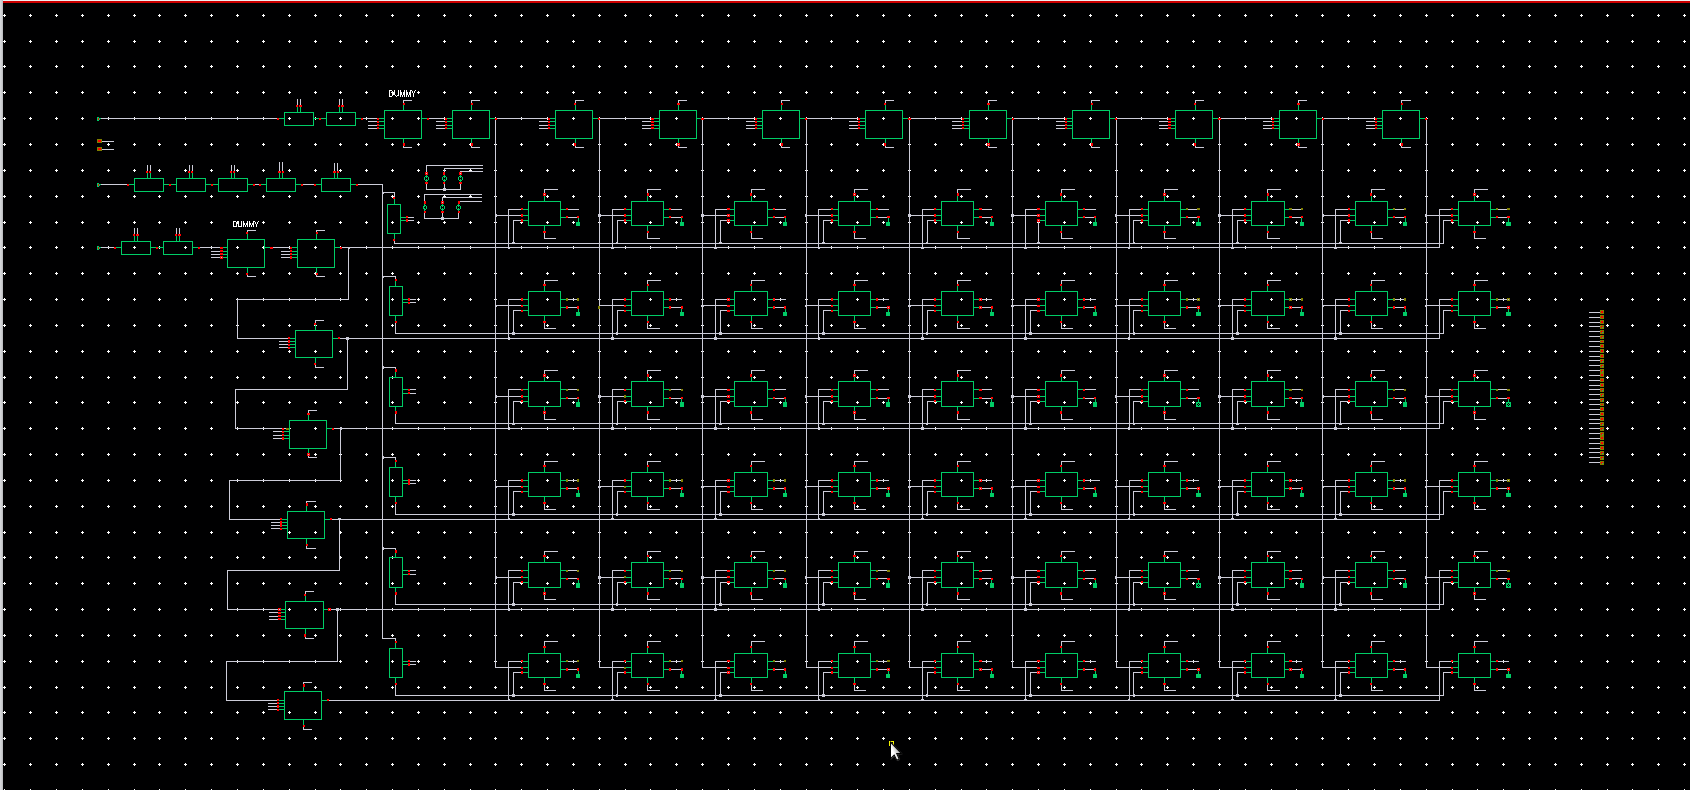
\includegraphics[width=0.95\textwidth]{figures/tdc_core_cadence.png}
\caption{\texttt{vernier2d/tdc\_core} as entered in Cadence Virtuoso: START
line across the top, STOP line down the left, and the $10\times6$ padded
latch matrix. The core contains 1120 active devices.}
\label{fig:core}
\end{figure}

The core (Fig.~\ref{fig:core}) instantiates 11 \texttt{delay\_tau1} and 7
\texttt{delay\_tau2} stages, 60 latches and the input buffer trees, and exposes
the course-mandated pins (RESET, START, STOP, $\Vdd$, GND, $Q_{1..31}$). The
six trim lines enter as static gate biases, standing in for configuration
bits. The total transistor width is $\sumw=\SI{1305.6}{\micro\meter}$:
\SI{1078.3}{\micro\meter} of active devices (1120 transistors) and
\SI{227.3}{\micro\meter} of MOSCAP (65 devices). The width budget is dominated
by the \texttt{delay\_tau1} drivers (\SI{451}{\micro\meter}) and the latch
NANDs (\SI{211}{\micro\meter}); the full breakdown is in
Appendix~\ref{app:sigmaw}.
